\let\negmedspace\undefined
\let\negthickspace\undefined
\documentclass[journal]{IEEEtran}
\usepackage[a5paper, margin=10mm, onecolumn]{geometry}
\usepackage{tfrupee}
\usepackage{float}

\setlength{\headheight}{1cm}
\setlength{\headsep}{0mm}

\usepackage{gvv-book}
\usepackage{gvv}
\usepackage{cite}
\usepackage{amsmath,amssymb,amsfonts,amsthm}
\usepackage{algorithmic}
\usepackage{graphicx}
\usepackage{textcomp}
\usepackage{xcolor}
\usepackage{txfonts}
\usepackage{listings}
\usepackage{enumitem}
\usepackage{mathtools}
\usepackage{gensymb}
\usepackage{comment}
\usepackage[breaklinks=true]{hyperref}
\usepackage{tkz-euclide}
\usepackage[latin1]{inputenc}
\graphicspath{{figs/}}
\usepackage{color}
\usepackage{array}
\usepackage{longtable}
\usepackage{calc}
\usepackage{multirow}
\usepackage{hhline}
\usepackage{ifthen}
\usepackage{lscape}
\usepackage{circuitikz}

\begin{document}

\bibliographystyle{IEEEtran}
\vspace{3cm}

\title{1.8.24}
\author{EE25BTECH11007- Aniket}
\maketitle
{\let\newpage\relax\maketitle}

\setlength{\intextsep}{10pt}

\textbf{Question}:\\
If $(a,b)$ is the mid-point of the line segment joining the point 
$\vec{A}$ $(10,-6)$ and $\vec{B}$ $(k,4)$ and $a-2b=18$, find the value of $a,b$ and the distance $\vec{AB}$.\\
\solution

% Start equation numbering here as (1), (2), ...
\setcounter{equation}{0}
\renewcommand{\theequation}{\arabic{equation}}

Let
\(\vec{A}=\myvec{x_1\\ y_1}\) and \(\vec{B}=\myvec{x_2\\ y_2}\).
By the (matrix) section formula, the point dividing \(\vec{A}\vec{B}\) in the ratio \(k:1\) is
\begin{equation}
R_{\text{int}}=\frac{1}{k+1}[\,\vec{A}\;\vec{B}\,]\myvec{1\\ k}.
\end{equation}

\medskip

With \(\vec{A}=\myvec{10\\-6}\) and \(\vec{B}=\myvec{k\\4}\) and \(\vec{O}=\myvec{a\\b}\) the midpoint (\(k=1\)) is
\begin{equation}
\vec{O}=\frac12[\,\vec{A}\;\vec{B}\,]\myvec{1\\1}
=\frac12\myvec{10 & k\\[2pt] -6 & 4}\myvec{1\\1}
=\frac12\myvec{10+k\\[2pt]-2}
=\myvec{\dfrac{10+k}{2}\\[6pt]-1}.
\end{equation}

Thus,
\begin{align}
a &= \frac{10+k}{2}, \quad b = -1 \tag{3}
\end{align}

Using the given condition $a - 2b = 18$:
\begin{align}
\frac{10+k}{2} - 2(-1) &= 18 \tag{4}\\
\frac{10+k}{2} &= 16 \tag{5}\\
k &= 22 \tag{6}
\end{align}

So,
\begin{align}
a = \frac{10+22}{2} = \boxed{16}, \quad b = \boxed{-1} \tag{7}
\end{align}

\textbf{Distance Between \(\vec{A}\vec{B}\):}
\[
D=\|\vec{A}-\vec{B}\| \tag{8}
\]
Where,
\[
\|\vec{A}-\vec{B}\|=\sqrt{(\vec{A}-\vec{B})^{\top}(\vec{A}-\vec{B})}. \tag{9}
\]

Given,
\[
\vec{A}=\myvec{10\\-6},\qquad \vec{B}=\myvec{22\\4}. \tag{10}
\]

Now using the values of \(\vec{A}\) and \(\vec{B}\),
\[
\vec{A}-\vec{B}=\myvec{10-22\\-6-4}=\myvec{-12\\-10}. \tag{11}
\]

Next,
\[
(\vec{A}-\vec{B})^{\top}(\vec{A}-\vec{B})=\myvec{-12&-10}\myvec{-12\\-10}. \tag{12}
\]

\begin{align}
\|\vec{A}-\vec{B}\|&=\sqrt{(-12)^2+(-10)^2} \tag{13}\\
      &=\sqrt{144+100} \tag{14}\\
      &=\sqrt{244} \tag{15}\\
      &=\boxed{2\sqrt{61}}. \tag{16}
\end{align}

\begin{figure}[H]
    \centering
    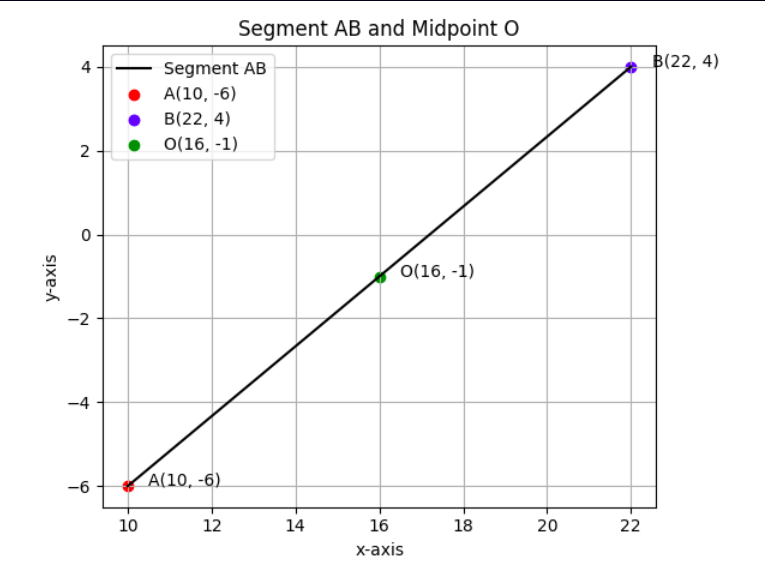
\includegraphics[width=\columnwidth]{figs/mg2.png}
\end{figure}

\end{document}
